\chapter{Verwendete Technologien}\label{cha:used-technologies}

\section{Over The Air Update (OTA)}\label{sec:ota}

\subsection*{Problemstellung}\label{sec:problem}
Mikrocontroller befinden sich, wenn sie sich in einem laufendem System befinden meist an ungünstigen Orten, an die man nur mit hohem Aufwand gelangt.
Bis jetzt musste man den Computer physisch mit einem Kabel mit dem Mikrocontroller verbinden um neue Firmware auf den Kontroller zu spielen.
OTA ermöglicht es den Mikrocontroller über das Netzwerk mit neuer Firmware zu versorgen, dabei muss der selektierte Microcomputer lediglich mit einem Wlan-Router verbunden sein und ein physisches Kabel wird überflüssig.

\subsection*{Wie OTA funktioniert}
Am wichtigsten ist es, dass man die Partitionstabelle an das ausgewählte Programm anpasst. 
Die Standard-Partitionstabelle ist je nach Hersteller anders. Um OTA zu ermöglichen ist es notwendig im Partitionstabelle mindestens eine, ausreichend große, OTA-Partition zu vergeben. Dabei ist es wichtig, dass diese Partition ausreichend Speicher für die gewünschte Firmware hat.

Bei dem OTA-Vorgang wird zuerst die Config-Datei, des jeweiligen Mikrocontrollers, ausgelesen. In dierser Config-Datei steht auch welches Firmware sich OTA herunterladen soll. Nun überprüft der Mikrocontroller ob die Firmware-Version des Servers neuer ist als die, die der Controller bereits besitzt, ist dies der Fall wird die neue Version heruntergeladen und der Mikrocontroller wird mit der aktuellen Version neu gestartet.

\subsection*{Implementation}
Die ausgewählte Struktur für die Diplomarbeit kann man im folgenden Bild sehr gut sehen.

\begin{figure}[H]
    \begin{center}
        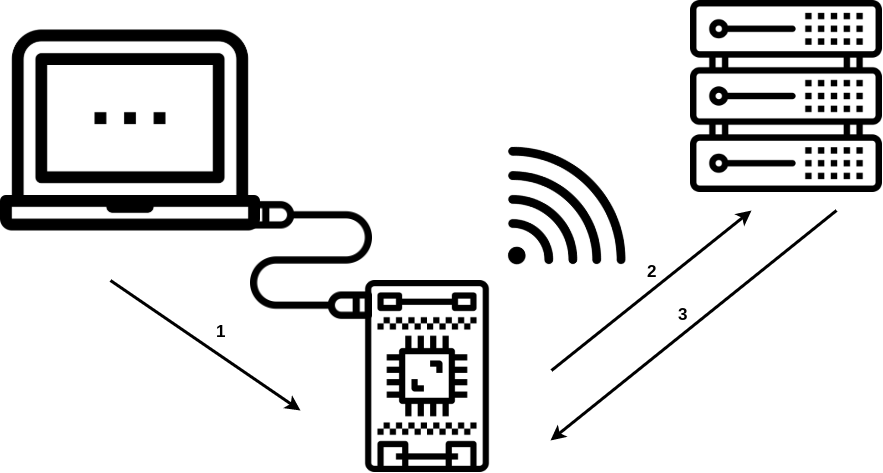
\includegraphics[scale=.5]{images/ota-explanation.png}
        \caption{OTA Erklärung (Quelle: eigene Darstellung)}
    \end{center}    
\end{figure}

\section{Mesh Netzwerk}\label{sec:mesh}

\section{Nodejs}\label{sec:nodejs}

Nodejs ist eine Laufzeit die auf der Javascript Engine von Chrome aufbaut. Nodejs wurde für das Backend des OTA Servers verwendet.

\subsection{Warum Nodejs?}

Java EE wurde hier nur als ein Beispiel gewählt. Folgendes gilt für jedes Framework das HTTP requests wie JavaEE behandelt. 
Bei der Überlegung welche Sprache bzw. welches Framework für das backend gewählt wird, war die Entscheidung sehr leicht.
Die Anforderungen des OTA Servers sind sehr einfach. Der Server dient nur zur Bereitstellung der Firmwares und beschreibende Informationen über die Firmwares selber.
Da dies nicht CPU intensiv ist sondern I/O intensiv, wurde in diesem Fall Nodejs gewählt.

\subsection{Event Loop}

\subsubsection{Was ist der Event Loop?}

Nodejs selber ist single-threaded deswegen ist der Event Loop einer der wichtigsten Bestandteile von Nodejs.
Der Event Loop erlaubt es nicht-blockenede I/O Operationen durchzuführen. Dies passiert durch die Abladung auf den Kernel von so vielen Operationen wie möglich.
\newline
\newline
Die meisten modernen Kernels sind multi-threaded. Das bedeutet, dass sie mehrere Operationen im Hintergrund unterstützen.

\subsubsection{Wie funktioniert der Event Loop?}

\begin{figure}[H]
    \begin{center}
        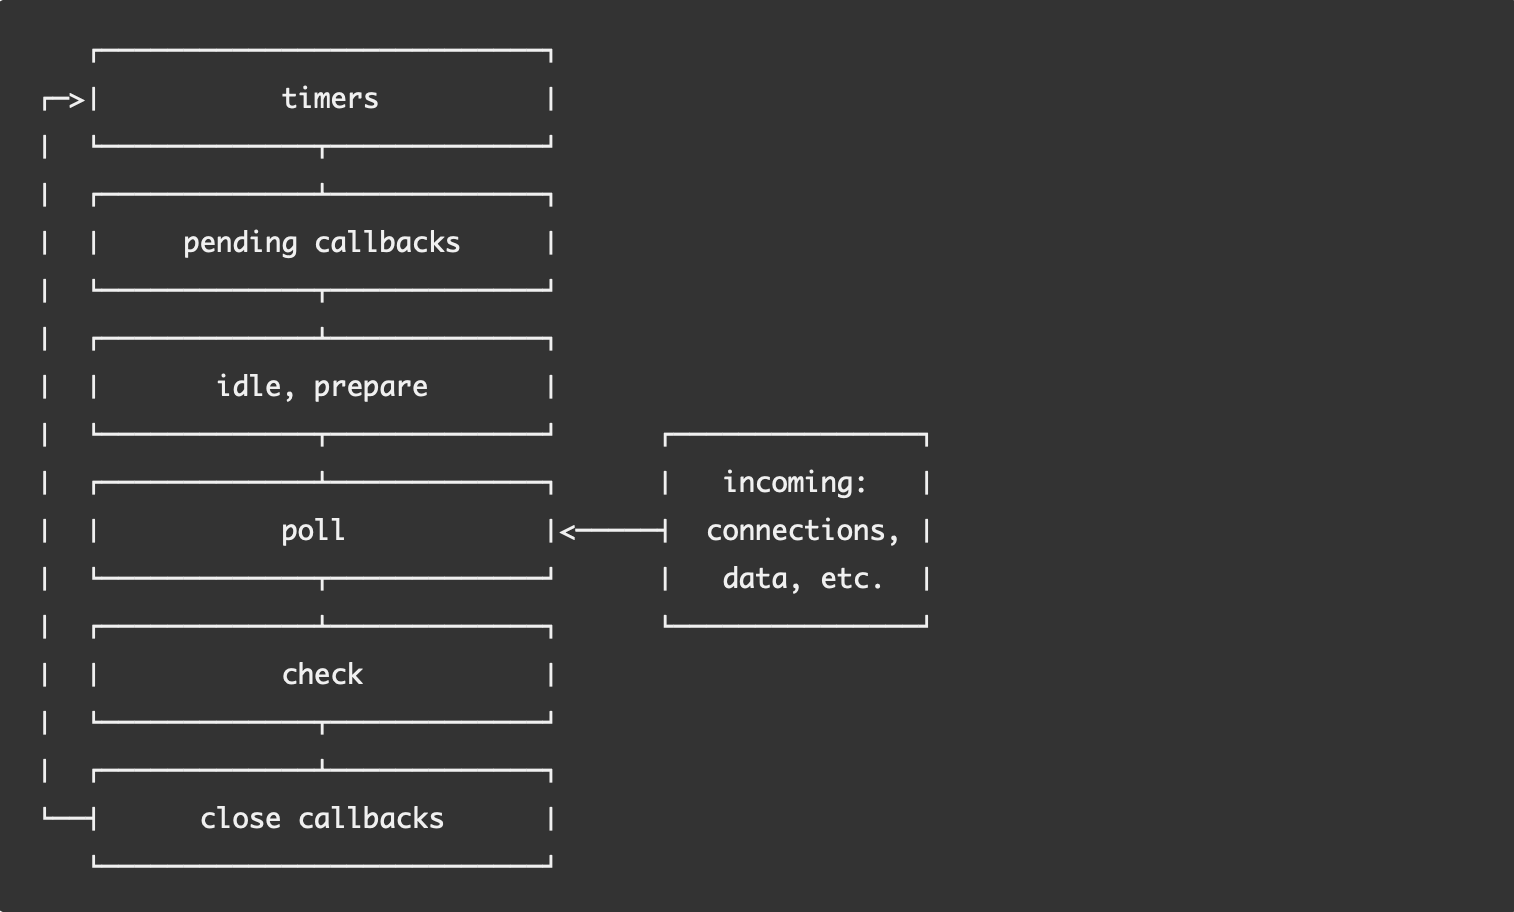
\includegraphics[scale=0.5]{images/nodejs_event_loop.png}
        \caption{Nodejs Event Loop \cite{nodejs_event_loop}}
    \end{center}
\end{figure}

Jeder Block im obigen Bild wird als Phase bezeichnet.
Jede Phase verfügt über eine First-In-First-Out-Warteschlange (FIFO-Warteschlange) mit auszuführenden Rückrufen. 
Während jede Phase auf ihre Weise etwas Besonderes ist, führt sie im Allgemeinen,
wenn die Ereignisschleife in eine bestimmte Phase eintritt, alle für diese Phase spezifischen Operationen aus und führt dann Rückrufe in der Warteschlange dieser Phase aus, 
bis die Warteschlange erschöpft ist oder die maximale Anzahl von Rückrufen ausgeführt hat. 
Wenn die Warteschlange erschöpft ist oder das Rückruflimit erreicht ist, wechselt die Ereignisschleife zur nächsten Phase und so weiter.
\newline
\newline
Da für jeden dieser Vorgänge möglicherweise mehr Vorgänge geplant werden und neue Ereignisse, 
die in der Abfragephase verarbeitet wurden, vom Kernel in die Warteschlange gestellt werden, 
können Abrufereignisse in die Warteschlange gestellt werden, während Abrufereignisse verarbeitet werden. 
Infolgedessen können lange laufende Rückrufe dazu führen, dass die Abfragephase viel länger als der Schwellenwert eines Timers läuft. 

\subsubsection{Phasen}

\begin{itemize}
    \item \textbf{timers:} In dieser Phase werden von setTimeout () und setInterval () geplante Rückrufe ausgeführt.
    \item \textbf{pending callbacks:} führt I/O Callbacks aus, die auf die nächste Iteration verschoben werden
    \item \textbf{idle, prepare:} wird nur intern verwendet
    \item \textbf{poll:} neue I/O Events abrufen; I/O bezogene Callbacks ausführen (fast alle mit Ausnahme von schließ Callbacks, die von Timers geplant werden, und setImmediate ()); Der Knoten wird hier gegebenenfalls blockiert
    \item \textbf{check:} setImmediate() Callbacks werden hier ausgeführt
    \item \textbf{close callbacks:} schließ Callbacks werden ausgeführt
\end{itemize}

Zwischen jedem Durchlauf des Event Loops prüft Nodejs, ob es auf asynchrone I/O oder Timer wartet, und fährt sauber herunter, wenn keine vorhanden sind.

\cite[Zitiert von der offizielen Nodejs Website]{nodejs_event_loop_how_does_it_work}

\section{Platform IO}\label{sec:platformio}

\section{ESP IDF Toolchain}\label{sec:platformio}

\section{Docker}\label{sec:docker}

\section{Docker Compose}\label{sec:docker-compose}

Docker-compose ist ein Tool zum Definieren und Ausführen von Docker-Anwendungen mit mehreren Containern. Mit Compose verwenden Sie eine YAML-Datei, um die Dienste Ihrer Anwendung zu konfigurieren. Anschließend erstellen und starten Sie mit einem einzigen Befehl alle Dienste in Ihrer Konfiguration. \cite{docker_compose_description}

\subsection{Docker Compose Beispiel}

\begin{figure}[H]
    \begin{center}
        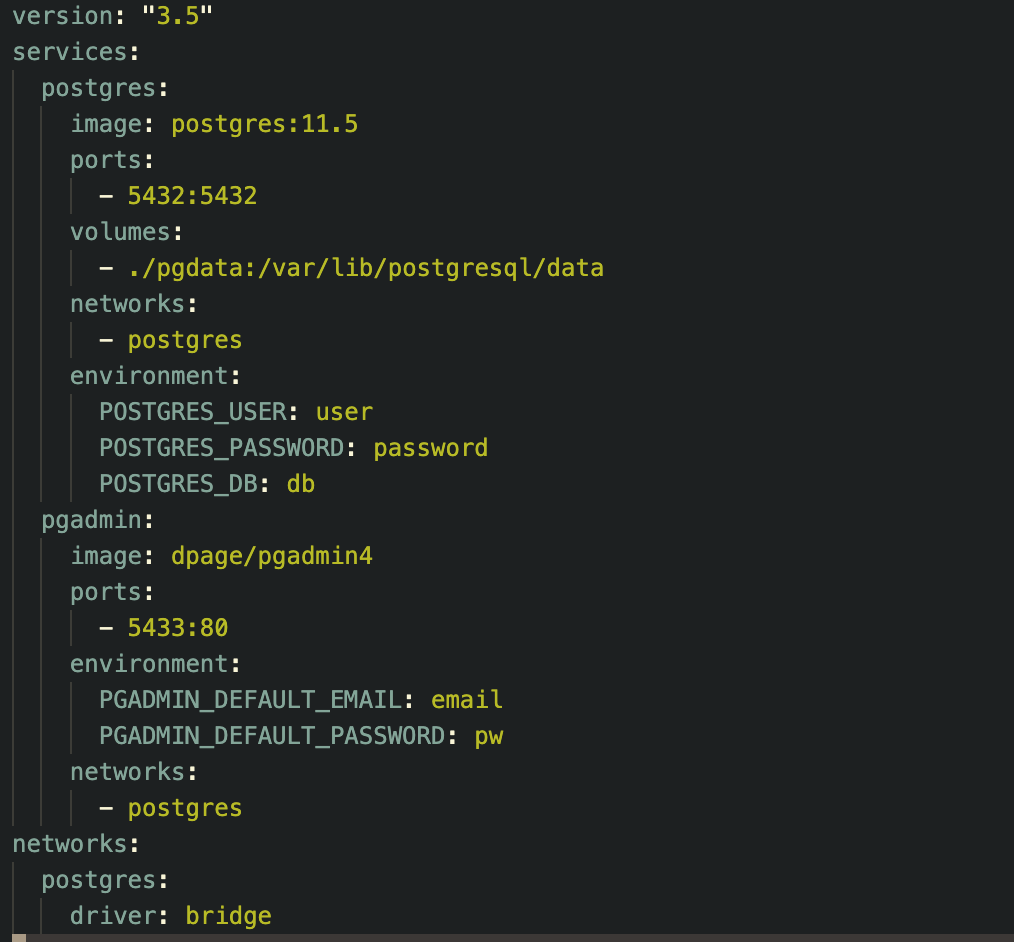
\includegraphics[scale=0.8]{images/docker_compose_example.png}
        \caption{Docker Compose Beispiel}
    \end{center}
\end{figure}

In der obigen Abbildung kann man das docker-compose.yml file von dem OTA Server sehen.

Die Struktur eines docker-compose files ist im Normalfall immer gleich. Am Anfang definiert man welche Version des Standards man verwendet und anschließend die verschiedenen Dienste. Der OTA Server benötigt nur 2 Dienste:

\begin{enumerate}
\end{enumerate}

\section{ESP IDF Utility lib}\label{sec:esp-idf-utility-lib}

\section{React}\label{sec:react}

\section{Yarn}\label{sec:yarn}

\section{Webpack}\label{sec:webpack}
